\documentclass[
portrait,
% landscape,
a0paper%,
% draft
]
{baposter}
%
% load packages
% already loaded some useful packages for figures, tables, layout and equations
% not all are needed to run this minimal example
\usepackage{graphicx}
\usepackage[percent]{overpic}
\usepackage[detect-weight]{siunitx}
\usepackage{tabto}
\usepackage{booktabs}
\usepackage{amsmath}
\usepackage{float}
\usepackage{multirow}
\usepackage{url}
\usepackage{enumitem}
\usepackage{qrcode}
% add additional packages you need here

% This required for proper figures caption work
\usepackage[font=small,labelfont=bf]{subcaption} % <-- changed to subcaption

\usepackage{multicol} % Required for multiple columns
\setlength{\columnsep}{1.5em} % Slightly increase the space between columns
\setlength{\columnseprule}{0mm} % No horizontal rule between columns

% Add your own packages.
%%% Math packages
\usepackage{physics, siunitx}
\usepackage{isomath}

%%% Bold symbols
\newcommand{\bv}{\vb*{v}}

%%% underbraces
\NewDocumentCommand{\myunderbracetext}{m}{\text{#1}\\} % for internal use
\NewDocumentCommand\myunderbrace{ O{\int} m >{\SplitList{\\}}m }
{% two mandatory arguments: 2 - formula and 3 - caption delimited by \\
    \underbrace{\vphantom{#1}#2}_{\substack{\ProcessList{#3}{\myunderbracetext}}}
}

% for now usig bibitem, but if you want ...
%\usepackage[backend=biber]{biblatex} 
%
% customizing 
\newlength{\mytextsize}
\newcommand\e{\cdot 10^}
\setlength{\unitlength}{1.0cm}
%
% define skoltech color  
\definecolor{skoltechgreen}{RGB}{102,217,44} %for text / color / logo
% fonts
\usepackage[scaled]{helvet}
\renewcommand*\familydefault{\sfdefault}
%
%
%##################################################################################
\begin{document}
%##################################################################################
\begin{poster}
{
  % options
  grid=false,%true,
  background=plain,
  bgColorOne=white,
  columns=6, % for flexibility changing 2/3 columns with columnspan
  eyecatcher=false,
  borderColor=skoltechgreen,
  headerColorOne=skoltechgreen, %white,
  headershade=plain,
  %headerColorTwo=white,
  headerborder=open,
  % for rectangular boxes change the next two options, rectangular header will cause left aligning of box title 
  textborder=rounded, %rectangle,
  headershape=rounded, %rectangle,
  headerfont=\bf\Large,
  boxshade=none,
  headerFontColor=white
}
{
  %eyecatcher ...
}
{
  %poster title
  % first put graphics for header
  \hspace*{-0.5mm}
  \begin{picture}(23.7, 3)
  \fboxsep0pt
  \put(-0.196, -0.6){\colorbox{skoltechgreen}{\rule[96pt]{675.82pt}{0pt}}}
  \thicklines
  % minipage box for title and authors
  \put(2.55, 2.35){
    \begin{minipage}[t][96pt]{0.75\textwidth}
    % centering
    \begin{center}
    % Title
    % use \LARGE instead of \Huge for long titles, you might need to modify distances or number of lines
    % for one line title
    %\ \vspace{0.15cm}\\
    %\huge\bf\color{white}\selectfont Single Line Title \vspace{0.4cm}\\ 
    % for two line title
    \huge\bf\color{white}\selectfont Effect of Solidification Shrinkage on Topography \\ 
    \huge\bf\selectfont Formation in Laser Surface Melting \vspace{0.15cm} \\ 
    \vspace{0.2cm}
    \small\underline{D.V. Panov}, O. A. Rogozin, O. V. Vasilyev.
    \end{center} 
  \end{minipage}}
  %  
  % some logo
  % left:
  %\put(0.32,-0.24){\includegraphics[height=75pt]{logos/LogoOutline-White.eps}}
  % right:
  \put(20.52,-0.24){
\includegraphics[height=75pt]{logos/Skoltech_CMT_log}}
  \end{picture} 
}
{
	%poster authors, already in title
}
{
	%logo, already in title
}
% in the following is here a simple example for two column layout with
% three boxes on the left: motivation, left box 1, left box 2 and
% two boxes on the right: right box 1, right box 2
%
\headerbox{Motivation}{name=motivation, column=0, row=0, span=3}{
  The topography after laser surface melting is the result of a combination of different physical phenomena. Mathematical modeling can be used to estimate the effect of thermophysical properties on the resulting topography. The most important phenomena such as capillarity, thermocapillarity, evaporation are considered in a number of studies. An important but most often neglected effect is the shrinkage during solidification. In the presented work an approach modelling the effect of shrinkage on the solidification is considered and the  results of numerical simulations are presented.
}
%
%
\headerbox{Mathematical model}{name=math_model, span=3, below=motivation, column=0}{
  Let us consider a domain consists of three phases such that:
  \[\rho = (1-\alpha) \rho_{\text{G}} + \phi \rho_{\text{L}} + (\alpha - \phi) \rho_{\text{S}},\]
  \[\rho h = (1 - \alpha) \rho_{\text{G}} h_{\text{G}} + \phi \rho_{\text{L}} h_{\text{L}} + (\alpha-\phi) \rho_{\text{S}} h_{\text{S}},\]
  where $\rho_{\text{P}}$ is the density of a given phase P, $h_{\text{P}}$ is the enthalpy of a given phase P, $\alpha$ is the volume fraction of metal and $\phi$ is the volume fraction of liquid metal.\\

  The system of governing equations for $\alpha$, $\bv$, $h$ can be written as follows:
  \begin{gather*}
    \partialderivative{\alpha}{t} +  \div (\alpha \bv) = \div \bv,
    \label{eq: advection_VOF}\\ 
    \div \bv = - \frac{(\rho_{\text{L}} - \rho_{\text{S}})D_t \phi + \phi D_t \rho_{\text{L}}}{\phi \rho_{\text{L}} + (1-\phi) \rho_{\text{S}}},
    \label{eq: mass_conservation}\\
    \begin{gathered}
        \pdv{\rho\bv}{t} 
        + \div (\rho \bv \otimes \bv)
        = 
        - \grad p
        + \grad \vdot \btau
        - \myunderbrace{K\alpha\frac{(\alpha-\phi)^2}{\phi^2 + \epsilon}\bv}{Brinkman penalization} 
        + \myunderbrace{\rho\bg}{gravity} \\
        - \myunderbrace{\gamma\qty(\div\bn_\alpha)\grad\alpha}{surface tension}
        + \myunderbrace{\dv{\gamma}{T}\qty(\bn_\alpha\cp\grad{T}\cp\bn_\alpha)|\grad \alpha|}{Marangoni force}
        - \myunderbrace{p_{\text{recoil}}(T)\grad \alpha}{recoil pressure},
    \end{gathered}\\
    \begin{gathered}
        \partialderivative{\rho h}{t} 
        + \div (\rho \bv h) 
        =
        \myunderbrace{\div k \grad{T}}{heat conductivity}
        + \myunderbrace{I_{\text{L}} |\grad \alpha|}{laser heat source}
        + \myunderbrace{Q_{\text{evap}}(T)|\grad \alpha|}{evaporation cooling}.
    \end{gathered}\label{eq: h_eq}
\end{gather*}

  \centering{
  \setcaptiontype{figure}
  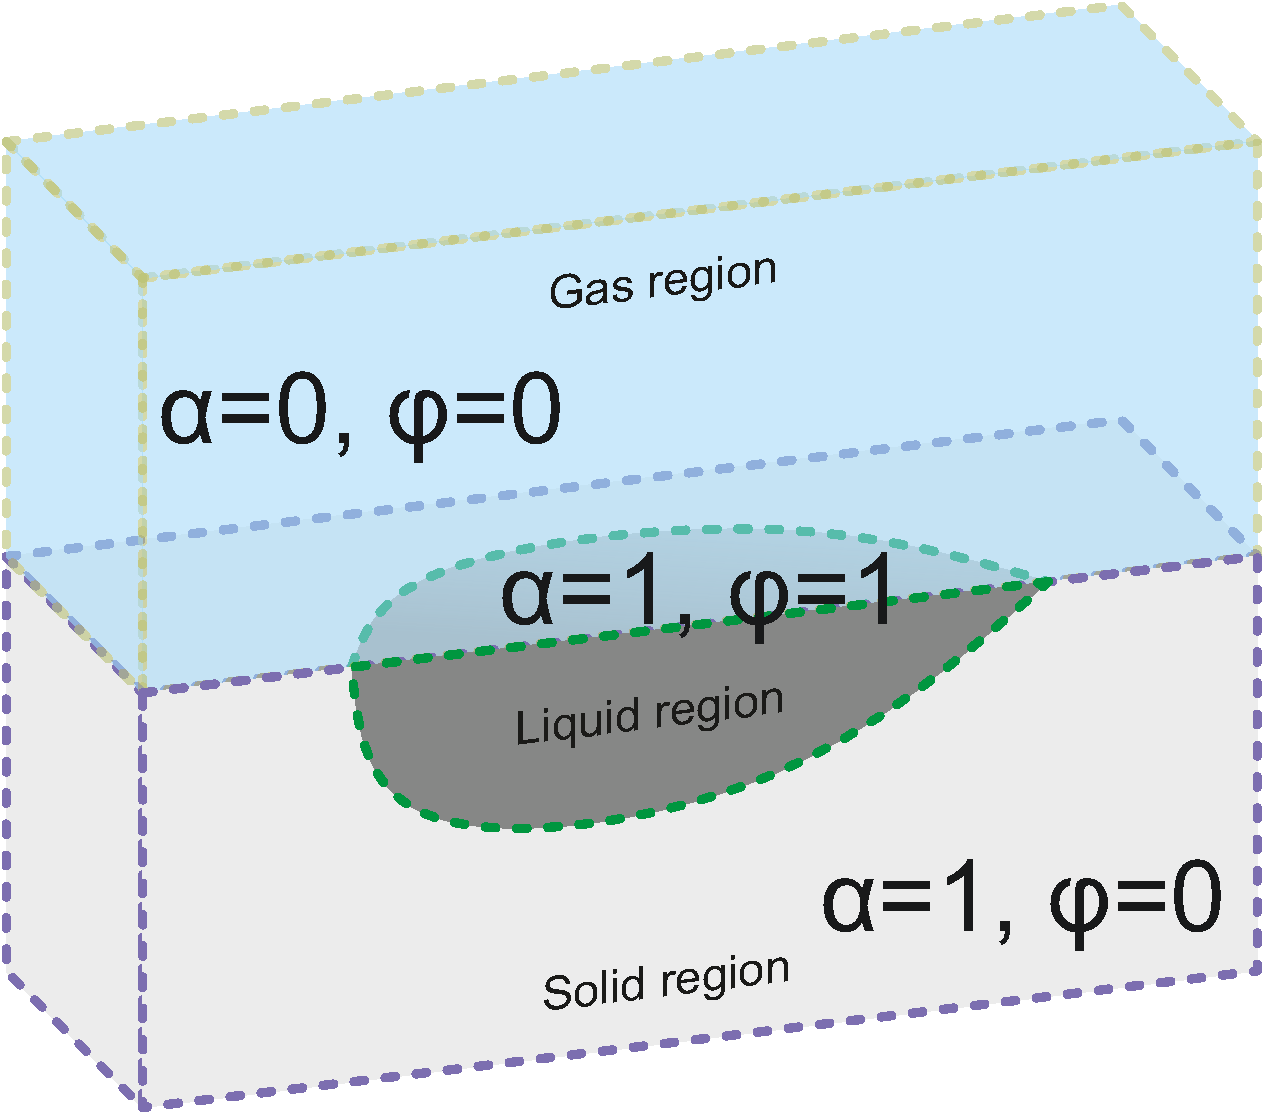
\includegraphics[width=0.4\linewidth]{pictures/3_phase_domain_alpha_phi.pdf}\\
  \caption{Schematic representation of the computational domain with the metal volume fraction $\alpha$ and the molten metal volume fraction $\phi$ distribution for different phases.}}\\
\hfill \\
\\
\raggedright {Details of the computational method and implementation:}
\begin{itemize}[noitemsep,topsep=0pt,parsep=0pt,partopsep=0pt, leftmargin=10pt]
  \item Finite Volume Method;
  \item Implicit Euler time integration;
  \item Volume fraction of metal $\alpha$ is treated with geometric Volume of Fluid method;
  \item Segregated solution;
  \item All the procedures are implemented in OpenFOAM\textregistered.
\end{itemize}

}
%
%
\headerbox{Conclusions}{name=conclusions, span=3, below=math_model, column=0}{
  \begin{itemize}[noitemsep,topsep=0pt,parsep=0pt,partopsep=0pt, leftmargin=10pt]
    \item An approach to incorporate metal density variability in mathematical model of melting process is presented;
    \item The difference in the final surface state of the considered numerical solutions shows the importance of considering the temperature compressibility of metal.
  \end{itemize}
}
\headerbox{References}{name=References, span=3, below=conclusions, column=0}{
  \begin{tiny}
 \begingroup 
 \renewcommand{\section}[2]{}
  \begin{thebibliography}{9}
      \vspace{-0.1cm}
	  \vspace{-0.1cm}

	    \bibitem{ref1}
      
      Pitscheneder W, DebRoy T, Mundra K and Ebner R 1996 Role of sulfur and processing variables on the temporal evolution of weld pool geometry during multikilowatt laser beam welding of steels \textit{Weld J.} \textbf{75} 71–80
       
        \vspace{+0.1cm}
    % \hfill \\
	\end{thebibliography} 
\end{tiny}
\endgroup
}
%
%
\headerbox{2D vertical solidification and pipe shrinkage}{name=al_solid, span=3, row=0, column=3}{
  \raggedright{Thermophysical properties are taken for pure aluminum. The surface tension is taken as a constant.  The rectangular domain size is $\Omega \in [0.8 \cross 10^{-3} \: \text{m}]^2$.}\\
  \centering{
  \setcaptiontype{figure}
  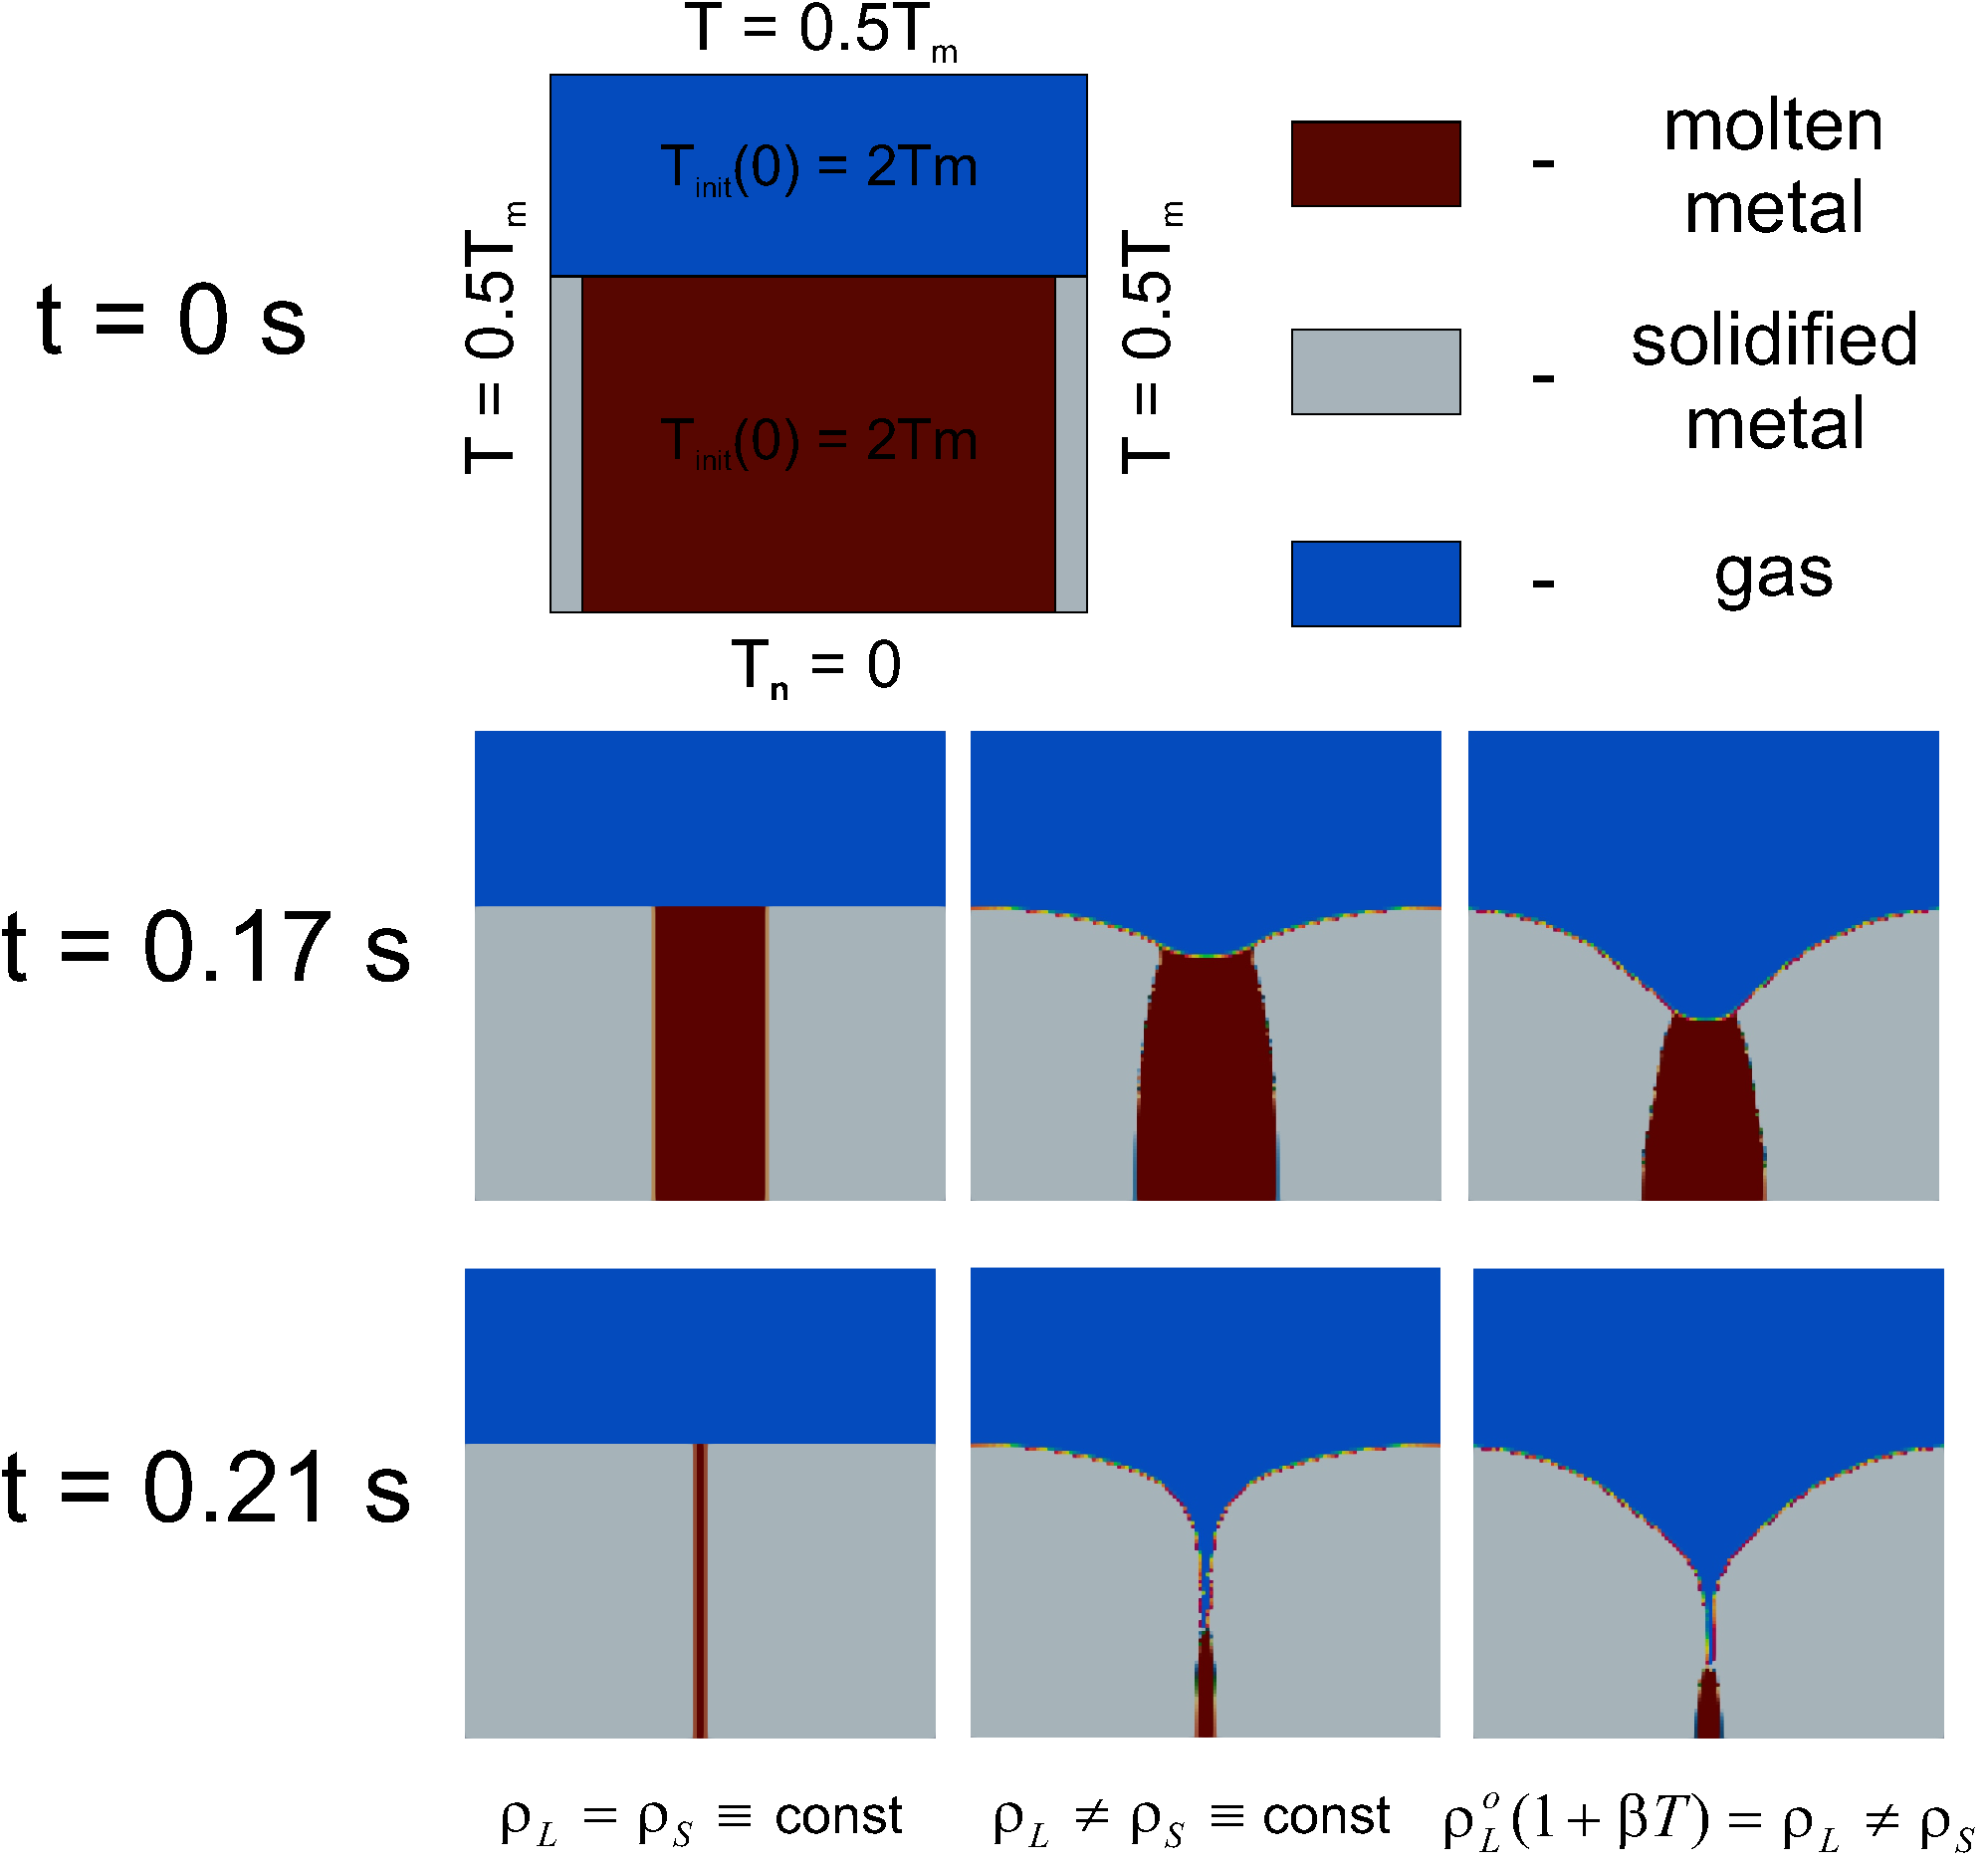
\includegraphics[width=0.855\linewidth]{pictures/Solidifcation at dfferent time.pdf}\\
  \caption{Aluminum vertical solidification problem and its numerical solution for phase distribution at different times for different cases of densities $\rho_L$ and $\rho_S$.}}\\
  \hfill \\
  In the case of a difference in density between solid and liquid phases, a kind of solidification crack develops. This phenomenon is known as ``pipe shrinkage'' in casting.
}
%
%
\headerbox{2D laser pulsed melting}{name=pulsed_melt, below=al_solid, span=3, row=0, column=3}{
  \raggedright{The results of the study on mathematical modeling of pulsed laser melting by Pitscheneder et al. are used as a benchmark [1]. A top-hat $\text{CO}_2$ laser beam with power of 5200 W irradiates at a point for 5 seconds.} \\
  \setcaptiontype{figure}
  \centering{
  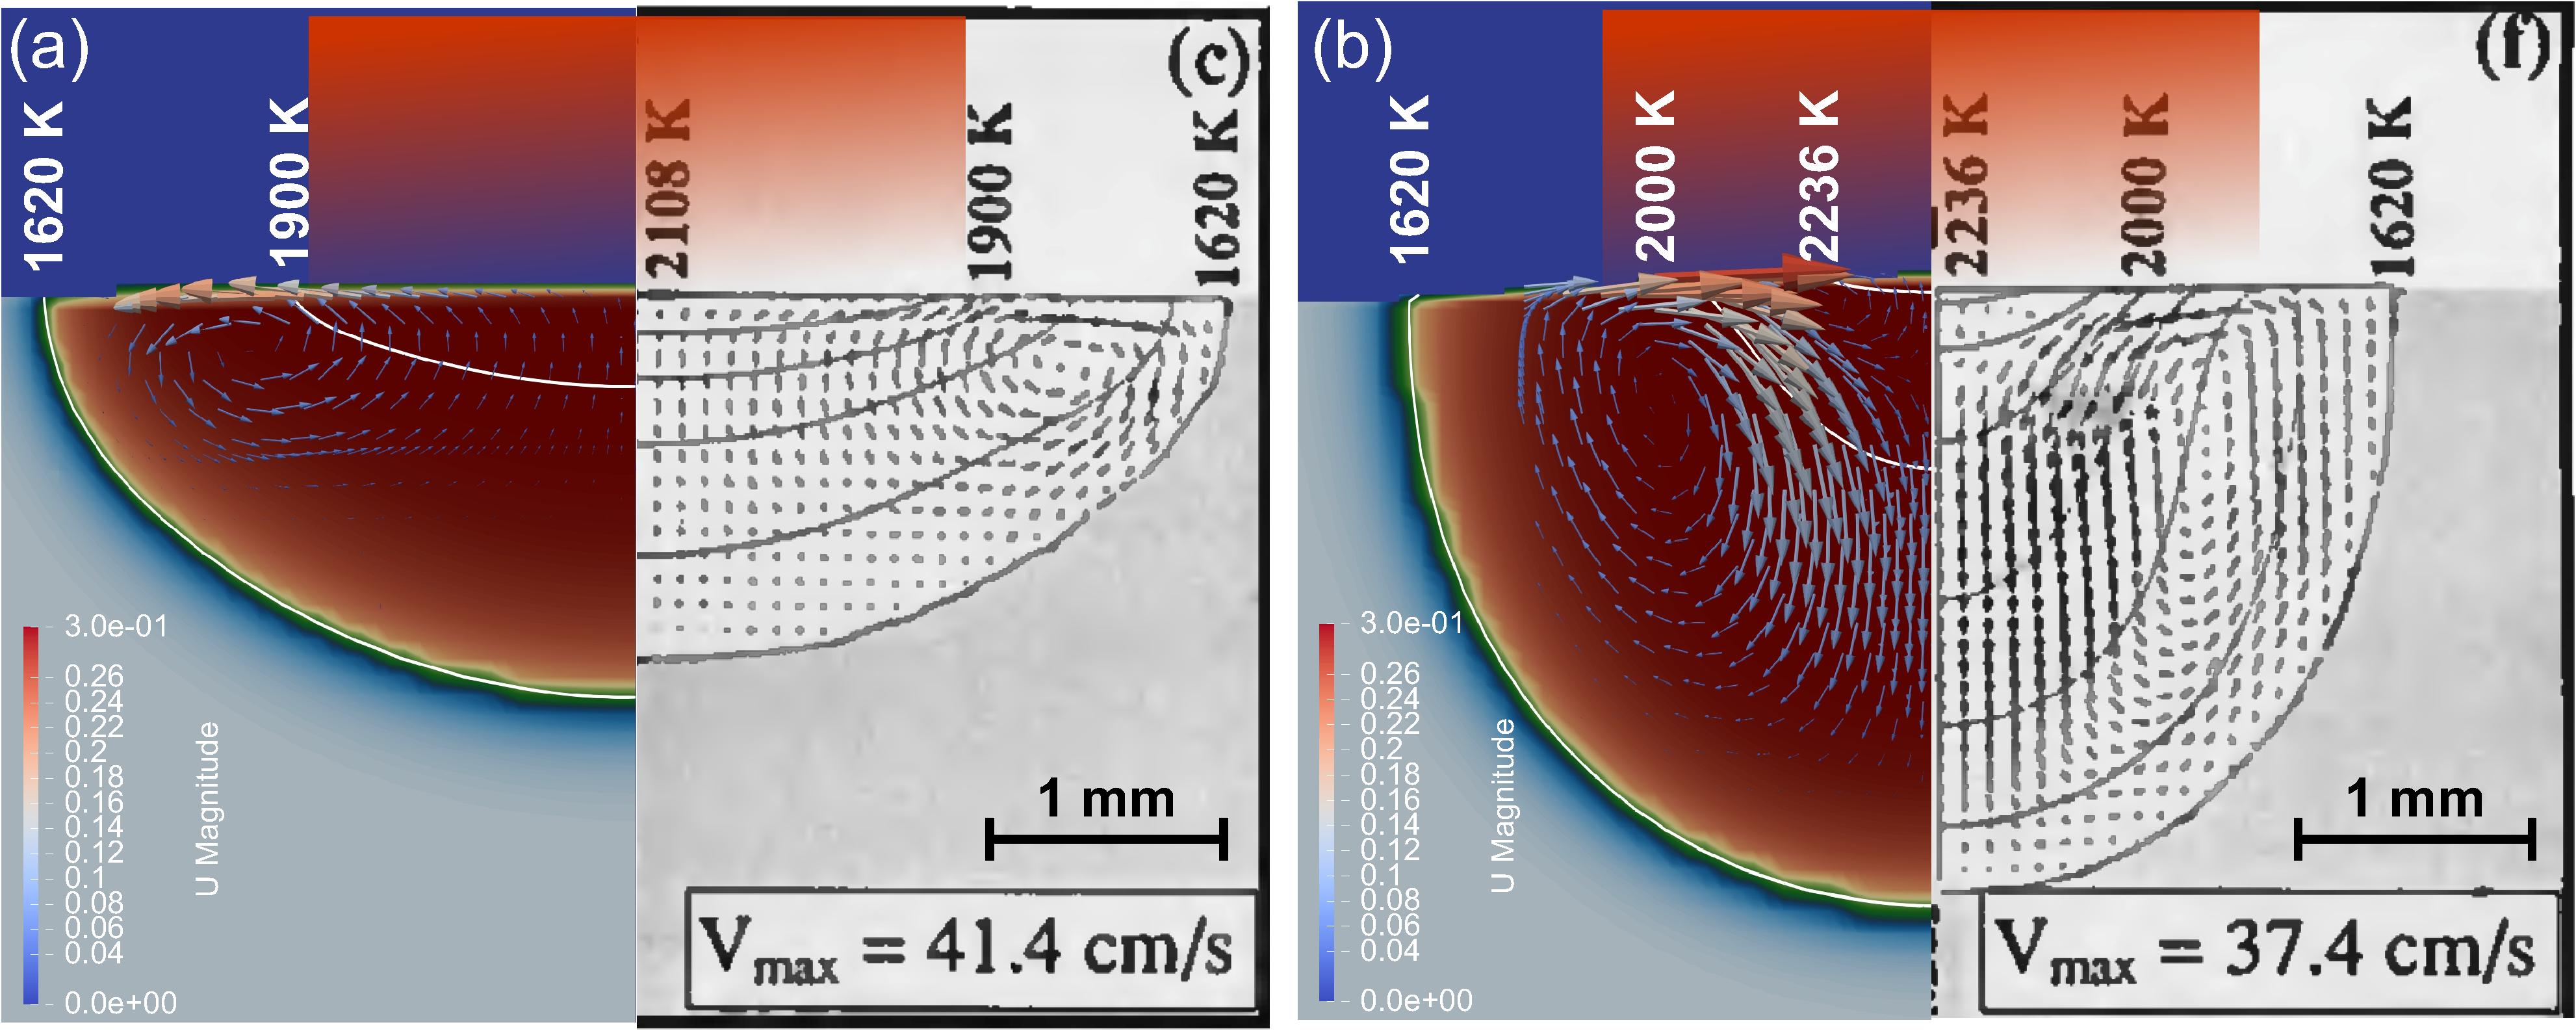
\includegraphics[width=0.908\linewidth]{pictures/Pitscheneder_sim_sim_cont.pdf}\\
  \caption{Comparison of numerically calculated molten metal fraction, temperature countours and velocity distribution for different sulfur concentrations of 20 ppm~(a) and 150 ppm~(b) in the presented work and in Pitscheneder et al. [1]}}\\
  \hfill \\
  \centering{
  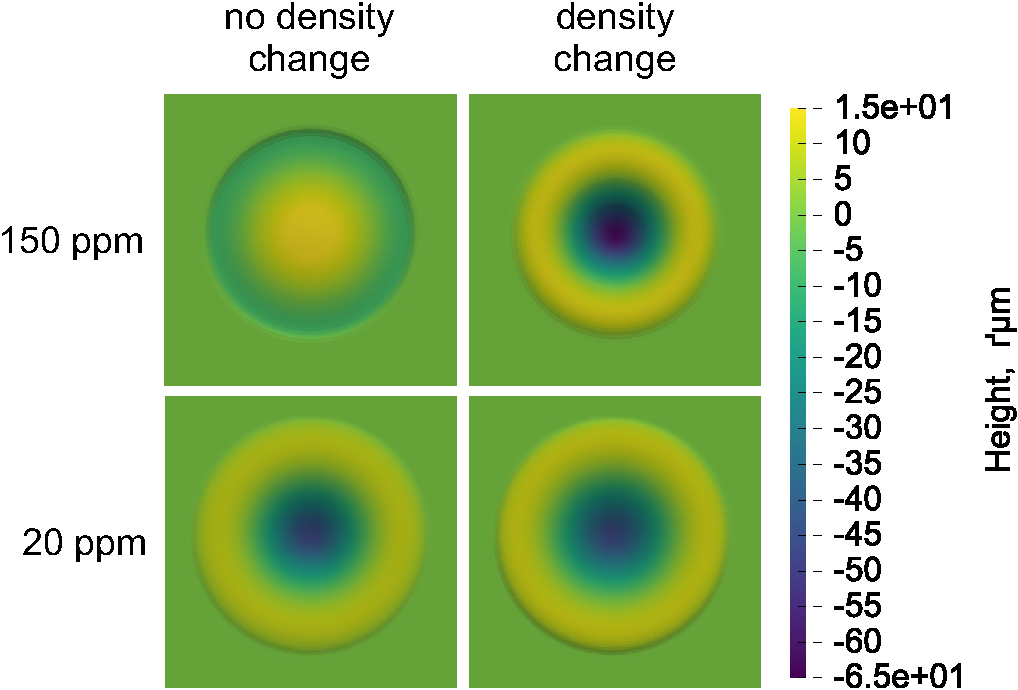
\includegraphics[width=0.611\linewidth]{pictures/single_point_melting_topography.pdf}\\
  \caption{Numerically calculated surface topography after solidification for various sulfur concentrations in case of constant and variable density.}}\\
  \hfill \\
  The final surface topography defines by Marangoni flow and solidification shrinkage.
}
% 
% 
% \headerbox{Summary and Outlook}{name=summary, span=3, below=pulsed_melt, above=foottext, column=3}{
%   \begin{itemize}[noitemsep,topsep=0pt,parsep=0pt,partopsep=0pt, leftmargin=10pt]
%     \item summary
%     \item outlook
%   \end{itemize}  
% }
%
%
\end{poster}
\end{document}
